
\textbf{一份按「判据能不能闭合」组织的综述（2025-01 — 2026-11）}


\begin{quote}\small
\textbf{数据快照}：2026-11-05 ｜ \textbf{纳入论文}：23 篇（core 15 / 旁证 8）｜ \textbf{来源时间跨度}：2025-03 至 2026-11 ｜ \textbf{主张}：12 条 ｜ \textbf{证据}：60 条（高置信 12 条）

\end{quote}

\begin{abstract}

2025 年以来，一类系统开始把「改推理系统」这件事交给模型自己：读代码、改调度、跑一遍端到端基准、看吞吐、再改。SpecPilot、SEIS、VibeServe 都属于这一类，它们常被称为「自我改进」甚至「递归自我改进（RSI）」。


本文要回答的问题比「它们有多快」更窄也更硬：\textbf{端到端层的循环用什么判据才敢说「改进了」，这些判据在哪里失效。}


本文核对了 2025 年 3 月至 2026 年 11 月的 23 篇论文（15 篇实现循环、8 篇提供判据或天花板），核心贡献有四。


\textbf{第一，端到端的被优化对象不是代码，是「系统设计 + 运行时状态」。} kernel 层优化的是一个可独立编译、独立计时、独立验算的程序；端到端层优化的是配置、调度策略、算法形状与运行时决策的混合体。同一个 kernel 的最优配置取决于 MoE 路由把 token 分到哪个专家上，而不只取决于 token 数{\scriptsize\texttt{[c-\hspace{0pt}object-\hspace{0pt}e2e]}}。因此端到端的判据必须同时覆盖吞吐、数值正确与部署约束三者。


\textbf{第二，端到端的「改进」必须写成统计命题。} 一次改动的典型幅度是几个百分点，而跨机器的绝对值漂移可以让同一个配置从 1.174 倍变成 1.0049 倍、用最差初稿作分母可以让同一个 kernel 从 2.03 倍变成 10.6 倍{\scriptsize\texttt{[c-\hspace{0pt}judge]}}。故晋级判据不能是点估计，只能是「增益的 95\% 下界同时超过最小实际增益与若干倍的系统自身噪声」{\scriptsize\texttt{[c-\hspace{0pt}judge]}}。SpecPilot 用 H100 上小于 0.1\% 的 stock 对 stock 噪声作参照，把门槛定在 1\%{\scriptsize\texttt{[c-\hspace{0pt}judge]}}。


\textbf{第三，「无损」不能用逐位相同，也不能用任务准确率。} 浮点归约顺序会翻转近 tie 的 argmax，故逐位相同会误杀；而注入一个 logit bias 后任务准确率几乎不动，故准确率会漏放。可行做法是把系统输出喂回精确引擎重打分、逐 token 比 argmax，再用「相对基线失配率的增量」与「大 margin 失配事件数」两条规则拒绝{\scriptsize\texttt{[c-\hspace{0pt}lossless]}}。


\textbf{第四，端到端层的主要风险不是搜不到，而是测不准。} 稻草人基线、绝对值不可迁移、任务饱和、基础设施缺陷四种失效模式，都会让循环「学到」一个不存在的改进{\scriptsize\texttt{[c-\hspace{0pt}measure]}}。而机制本身还会反号：批处理下 24 节点树在 FP8 目标上掉 14.9\%，24 位置块在 BF16 上掉 9.9\%，TLV 掉 13\%{\scriptsize\texttt{[c-\hspace{0pt}boundary]}}。


\textbf{结论：端到端层目前是「判据已经工程化的自动优化」，不是递归自我改进。} 可累积的部分是机制级的记忆条目，不是权重；而脚手架自改进的实证只有「7 次可评估改动里 3 次有效、4 次无效」{\scriptsize\texttt{[c-\hspace{0pt}harness]}}。


\textbf{关键词}：推理系统；投机解码；自我改进；反馈信号；无损判定；测量可信；端到端收益


\end{abstract}
\section{引言：两个都很快的系统，和两个都不能直接信的倍数}

\subsection{同一时期的两组数字}

2026 年 11 月，SpecPilot 报告：在一个 H100 上，单请求场景把相对自回归的解码加速比从 stock 的 4.46 倍提到 10.87 倍，批处理场景从 1.94 倍提到 3.93 倍，对 stock 的 sealed final 增益是 2.13 倍{\scriptsize\texttt{[c-\hspace{0pt}gain]}}{\scriptsize\texttt{[c-\hspace{0pt}gain]}}{\scriptsize\texttt{[c-\hspace{0pt}gain]}}。


同年 10 月，SEIS 报告：把整个 mini-sglang 引擎交给 agent 自演化，吞吐达到原实现的 3.27 倍，并在单请求负载上超过 vLLM、TensorRT-LLM 与 SGLang{\scriptsize\texttt{[c-\hspace{0pt}gain]}}。


这两个数字不能放在一起排序。前者是「相对同一引擎上一个被反复调优过的配置」，后者是「相对一个教学用引擎」。这正是本文的起点：\textbf{端到端层的数字不是一把尺子，而是一组各自带口径的量。}


\subsection{本文要检验的假设}

本文的假设只有一句：


\begin{quote}\small
端到端层的瓶颈不是「测不到速度」，而是\textbf{测到的速度不足以支撑判定}。

\end{quote}

若成立，则端到端层的方法学创新应集中在判据——配对运行、置信下界、无损定义、注入故障验证——而不是搜索算法本身。若某个系统的增益主要来自机制，判据只是包装，这条假设即失效。


第 7 章给出的四种失效情形是它的边界，第 8 章用脚手架自改进的实证对它做一次反证。


\subsection{纳入标准与数据来源}

\begin{itemize}
  \item \textbf{时间}：2025-03 至 2026-11（最早一篇入选为 2025-03-06；检索下限设 2025-01）
  \item \textbf{检索}：arXiv 官方 API，五组检索式（投机解码 / 服务系统 / 算法发现 / 量化 / 循环）共 23 条式子，去重后 1403 篇候选，脚本 \texttt{fetch\_serving.py} 可复现
  \item \textbf{筛选}：core 必须实现一个「agent 改动端到端推理链路并拿到端到端反馈」的循环，且给出可核对的实验；旁证提供判据的一半（测量方法、成本模型或天花板）
  \item \textbf{排除}：只改单个 kernel 的工作（已由另一篇归档处理）、纯模型训练效率、以及只在摘要里给倍数而无判据描述的工作
\end{itemize}

\sym{⚠}{} \textbf{两个必须声明的局限}：


\begin{enumerate}
  \item 本文所有数字都是二手，可逐条点回原文；但\textbf{本文没有跑任何实验}。
  \item 15 篇 core 里 2 篇的关键数字只在摘要中出现（locator 标 \texttt{abstract}），其余为全文。
\end{enumerate}

\section{被优化的对象：端到端与 kernel 层的结构差异}

\subsection{三层对象，三种判据}

把「端到端推理优化」拆开看，被优化的对象至少有三类，它们的判据强度递减：


\begin{table*}[t]
\centering
\footnotesize
\setlength{\tabcolsep}{4pt}
\caption{三层对象与判据：越往下，正确性判据越像阈值而不是等式}
\label{tab:1}
\begin{tabular}{llll}
\toprule
层 & 被优化的是什么 & 正确性判据 & 性能判据 \\
\midrule
kernel / 算子 & 一段可独立编译的 GPU 程序 & allclose + 隐藏测试集 & 稳健计时 \\
端到端 / 服务 & 系统设计 + 运行时状态 & 无损判据 + 下游任务 & 吞吐 / 延迟 / SLO \\
配置 / 容量 & 并行、精度、调度参数 & 与参考引擎输出一致 & 代理模型预测 + 实测校准 \\
量化 / 压缩 & 权重与 KV 的表示 & perplexity / KL / 准确率阈值 & 精度-吞吐前沿 \\
\bottomrule
\end{tabular}
\end{table*}

\subsection{为什么端到端不等于 kernel 的放大}

有一条来自源头的观察可以直接引用：\textbf{一个更快的微基准 kernel，在把 dispatch、显存分配、同步、批处理与通信都算进去之后，未必提高服务吞吐}{\scriptsize\texttt{[c-\hspace{0pt}object-\hspace{0pt}e2e]}}。


更具体地，端到端时间里有一部分完全不在 kernel 内部：在 TensorRT-LLM 上 profiling Qwen2.5-1.5B 显示，仅 kernel 启动开销就占端到端推理时间的 14.6\%{\scriptsize\texttt{[c-\hspace{0pt}object-\hspace{0pt}e2e]}}。


\subsection{运行时状态：一个必须先说的反例}

MoE 层给出了最干净的反例：serving 系统通常按批大小离线 autotune kernel 配置，但 MoE 的路由决定 token 如何分到专家与 GPU 上，\textbf{最优配置取决于这个分布而不只取决于 token 数}{\scriptsize\texttt{[c-\hspace{0pt}object-\hspace{0pt}e2e]}}。同一篇工作报告，在专家并行下按每张 GPU 实际 token 分布选配置，比沿用离线 autotune 的选择最多快 1.45 倍{\scriptsize\texttt{[c-\hspace{0pt}boundary]}}。


这条反例的含义是：端到端的「对象」包含运行时状态，而这种状态在离线时不可知。故端到端的循环必须在运行时闭合，不能只在部署前闭合。


\section{晋级判据：为什么必须是统计命题}

\subsection{判据的三个构件}

把端到端层的判定拆开，至少有四件不同的事要回答，缺一件循环就退化成「多试几次」：


\begin{table*}[t]
\centering
\footnotesize
\setlength{\tabcolsep}{4pt}
\caption{四类判据各回答什么：它们不能互相替代}
\label{tab:2}
\begin{tabular}{lll}
\toprule
判据层 & 回答什么 & 本主题的实例 \\
\midrule
成本模型 & 该往哪优化 & ceiling 三分之积 \\
晋级判据 & 是否真的更好 & 配对运行 + 95\% 下界 \\
无损判据 & 是否还正确 & token forcing + 两条拒绝规则 \\
成本核算 & 这么做值不值 & GPU-小时 vs 穷举基线 \\
\bottomrule
\end{tabular}
\end{table*}

\subsection{配对运行：把机器差异从分母里去掉}

SpecPilot 的做法值得逐字描述：\textbf{控制器是 agent 可以调用但不能修改的脚本}，它在配对运行中把候选与当前最优同时跑在同一批请求上、并在两次运行之间交换 GPU，以此计时{\scriptsize\texttt{[c-\hspace{0pt}judge]}}。


「交换 GPU」这个细节是判据的一部分，不是工程洁癖：它把 GPU 之间的系统差异变成了配对内部可抵消的量。


\subsection{下界对噪声：门槛怎么定}

晋级条件是：\textbf{增益的 95\% 下界同时超过 1\% 与两倍的 stock 对 stock 噪声}；若输出与当前最优不一致，门槛抬到约 3\%{\scriptsize\texttt{[c-\hspace{0pt}judge]}}。


这个门槛不是拍的。H100 单请求上 stock 对 stock 的噪声小于 0.1\%{\scriptsize\texttt{[c-\hspace{0pt}judge]}}，故实际门槛接近 1\%；而单条改动的典型量级是 1.06-\hspace{0pt}1.08 倍，正是为这种幅度设计的。


\subsection{为什么点估计一定不够}

两组数字说明点估计为什么不够用。


第一组来自跨机器：同一个配置在一台机器上交付 1.174 倍，在另一台上只有 1.0049 倍{\scriptsize\texttt{[c-\hspace{0pt}judge]}}。这意味着「某配置快 17\%」这句话在换机器之后会变成「快 0.5\%」，而后者已经在噪声里。


第二组来自基线选择：用最差初稿作分母，同一个 gelu tuning kernel 可以读出 10.6 倍；换成搜索实际起步的诚实基线，只有 2.03 倍{\scriptsize\texttt{[c-\hspace{0pt}judge]}}。两者相差五倍，而 kernel 一个字都没改。


\section{无损判据：为什么「逐位相同」和「准确率不降」都不行}

\subsection{两种都会错的判据}

逐位相同会误杀：浮点归约顺序会翻转近 tie 的 argmax，而这在正确实现里也会发生。


准确率不降会漏放：给每第 7 个 vocab id 在 2048 token 之后加一个 logit bias，任务准确率几乎不动，但输出已经系统性偏离。


\subsection{可行定义：精确 pass 的 argmax}

SpecPilot 的定义是：每个被接受的 token 都等于一次\textbf{精确权重} pass 的 argmax，且该 pass 的路径包含它。实现上是 teacher forcing——把系统的输出喂回 stock 引擎、用 FP32 LM head 重打分、逐 token 比对 argmax{\scriptsize\texttt{[c-\hspace{0pt}lossless]}}。


这个定义的关键在于它有基线：stock 自身在 0.72\% 的 token 上失配，几乎都是近 tie{\scriptsize\texttt{[c-\hspace{0pt}lossless]}}。故判据不是「零失配」，而是「不比 stock 更差」。


\subsection{两条拒绝规则}

\textbf{速率规则}：失配率高出 stock 超过 0.5 个百分点且 95\% 置信{\scriptsize\texttt{[c-\hspace{0pt}lossless]}}。


\textbf{事件规则}：margin 大于两倍近 tie 阈值的「大 margin 失配」经二项检验显著多于 stock{\scriptsize\texttt{[c-\hspace{0pt}lossless]}}。


速率规则抓系统性的普遍偏移，事件规则抓少量但严重的偏离——后者才是真正会改变语义的那一类。


\subsection{另一条路：三道数值门 + 下游门}

SEIS 走的是另一条路：数值门要求 perplexity 相对差在 5\% 以内{\scriptsize\texttt{[c-\hspace{0pt}lossless]}}，之下再叠一道下游任务门（GSM8K 与合成检索），理由写得很直白——数值差异会沿步累积{\scriptsize\texttt{[c-\hspace{0pt}lossless]}}。


\begin{table*}[t]
\centering
\footnotesize
\setlength{\tabcolsep}{4pt}
\caption{两种系统的无损判定对比：一个用统计检验，一个用阈值 + 下游兜底}
\label{tab:3}
\begin{tabular}{llll}
\toprule
系统 & 数值门 & 下游门 & 统计门 \\
\midrule
SpecPilot & exact pass 的 argmax & sealed final 未见请求 & rate rule + event rule \\
SEIS & perplexity 5\% / KL 0.05 & GSM8K + 检索任务 & —（无显式统计门） \\
\bottomrule
\end{tabular}
\end{table*}

两者的差别值得注意：SpecPilot 的判据是\textbf{比较式}的（相对 stock 的失配率增量），SEIS 的判据是\textbf{绝对式}的（阈值）。比较式的优点是自带基线，缺点是需要一个可信的 stock；绝对式的优点是简单，缺点是在不同模型上阈值要重调。


\section{成本模型：把「该往哪优化」变成可重算的因子}

\subsection{ceiling 的用途不是预测倍数}

SpecPilot 的成本模型做的是：\textbf{把实测性能与估计天花板比较，定位速度丢在哪里}{\scriptsize\texttt{[c-\hspace{0pt}ceiling]}}。


天花板被分解成三个因子的乘积，故每一项都可单独重算{\scriptsize\texttt{[c-\hspace{0pt}ceiling]}}：更好的树能多收多少 token、已计入 profile 的 kernel 离 byte floor 多远、profile 之外的开销还有多少。


\subsection{因子排序会变，这才是重点}

若天花板只是一个数，那么每轮都会指向同一个最大项。实际做法是每轮重算、按当前最大因子开方向{\scriptsize\texttt{[c-\hspace{0pt}ceiling]}}。


这不是形式主义。有一组同系统内的对照说明了它的价值：不使用 ceiling 排序的单 agent 版本，三轮只到 1.34 倍，而 SpecPilot 到 2.13 倍{\scriptsize\texttt{[c-\hspace{0pt}ceiling]}}。差别不在模型也不在预算，而在对照始终盯着最显眼的瓶颈。


\subsection{另一条路：用性能模型替代 profiling}

AIConfigurator 把同一件事做到了产业界更关心的位置：不跑 GPU、只用性能模型在配置空间里搜索，报告在 dense 模型上最多提升 40\%、MoE 上最多 50\%{\scriptsize\texttt{[c-\hspace{0pt}ceiling]}}。


它的代价也清楚：搜完 339 个配置用 0.52 秒，而同样的事用 GPU 实测要 24.4 小时{\scriptsize\texttt{[c-\hspace{0pt}gain]}}。这是「代理模型换实测」最干净的一笔账。


\section{增益与代价}

\subsection{把数字并列，但标清口径}

把本文核到的七条端到端增益并列，第一条就该看见的事不是大小，而是\textbf{它们不在同一把尺子上}：


\begin{itemize}
  \item 对\textbf{自回归}的加速：SpecPilot 单请求 10.87 倍、批处理 3.93 倍{\scriptsize\texttt{[c-\hspace{0pt}gain]}}。
  \item 对\textbf{某个既有系统}的加速：SpecPilot 对 stock 2.13 倍{\scriptsize\texttt{[c-\hspace{0pt}gain]}}、SEIS 对 mini-sglang 3.27 倍{\scriptsize\texttt{[c-\hspace{0pt}gain]}}、VibeServe 对调优后的 SGLang 2.30 倍、跨模型编译每轮几何均值 1.37 倍{\scriptsize\texttt{[c-\hspace{0pt}gain]}}。
  \item 对\textbf{默认配置}的提升：AIConfigurator 在 dense 模型上最多 40\%{\scriptsize\texttt{[c-\hspace{0pt}ceiling]}}。
\end{itemize}

三类分母的差别不是修辞。以 SpecPilot 自己为例：同一个系统，对自回归是 10.87 倍，对 stock 只有 2.13 倍——因为那个 stock 本身已经是每步 4.25 个 token 的调优配置{\scriptsize\texttt{[c-\hspace{0pt}gain]}}。\textbf{拿 10.87 去和别人的 2.13 比，等于把「别人的起点有多高」这件事从分母里删掉了。}


\begin{figure*}[t]
\centering
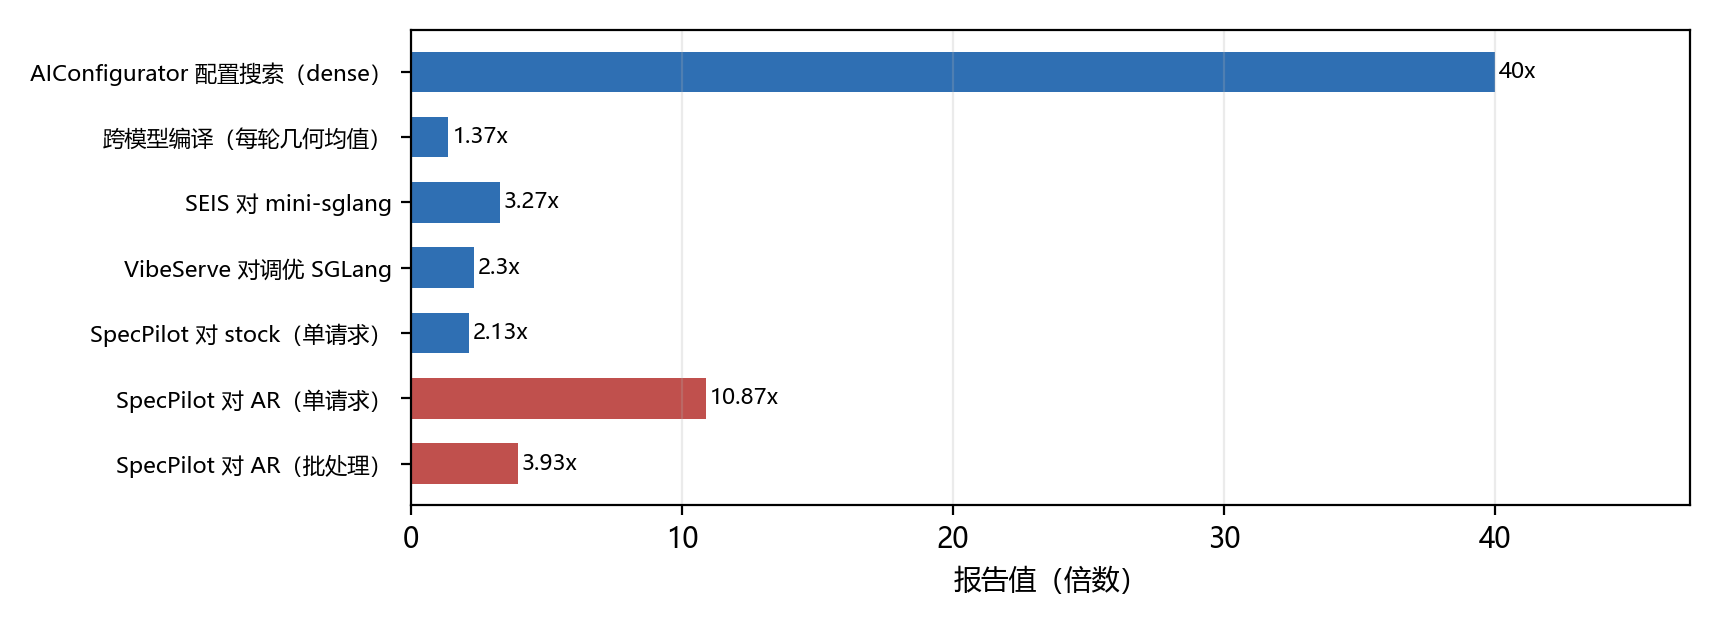
\includegraphics[width=0.86\textwidth]{../figures/fig1_gain.png}
\caption{图 1　端到端报告增益与口径差异。红色为「相对自回归」，蓝色为「相对某个既有系统」——两者分母不同，不能混读。}
\label{fig:1}
\end{figure*}

\subsection{为什么这个区间不能当排序}

三条理由，每条都有证据：


\begin{enumerate}
  \item \textbf{分母不同}：对自回归与对 stock 是两个分母，后者的 stock 已经被调优过（SpecPilot 自己指出 stock 的 4.46 倍只对应每步 4.25 个 token）{\scriptsize\texttt{[c-\hspace{0pt}gain]}}。
  \item \textbf{场景不同}：单请求与批处理差一倍以上，同一系统在两种场景下分别是 10.87 与 3.93{\scriptsize\texttt{[c-\hspace{0pt}gain]}}{\scriptsize\texttt{[c-\hspace{0pt}gain]}}。
  \item \textbf{机器不同}：同一模型在 H100 与 RTX PRO 6000 上的最优 stock 配置本身就不同{\scriptsize\texttt{[c-\hspace{0pt}gain]}}。
\end{enumerate}

\subsection{循环本身多贵}

这是最容易被省掉的一段，但它是结论的一部分。


单轮 7-\hspace{0pt}20 小时、20-\hspace{0pt}86 GPU-小时{\scriptsize\texttt{[c-\hspace{0pt}cost]}}；十三轮合计 164 小时与 530 GPU-小时，产生 486 个代码改动、晋级 54 个{\scriptsize\texttt{[c-\hspace{0pt}cost]}}。


作为对照：把本文所引研究里的配置候选穷举一遍约需 25,000 GPU-小时{\scriptsize\texttt{[c-\hspace{0pt}cost]}}，而代理模型在 172 个配置上的 TPOT 中位误差是 8.1\%{\scriptsize\texttt{[c-\hspace{0pt}cost]}}。


\begin{figure*}[t]
\centering
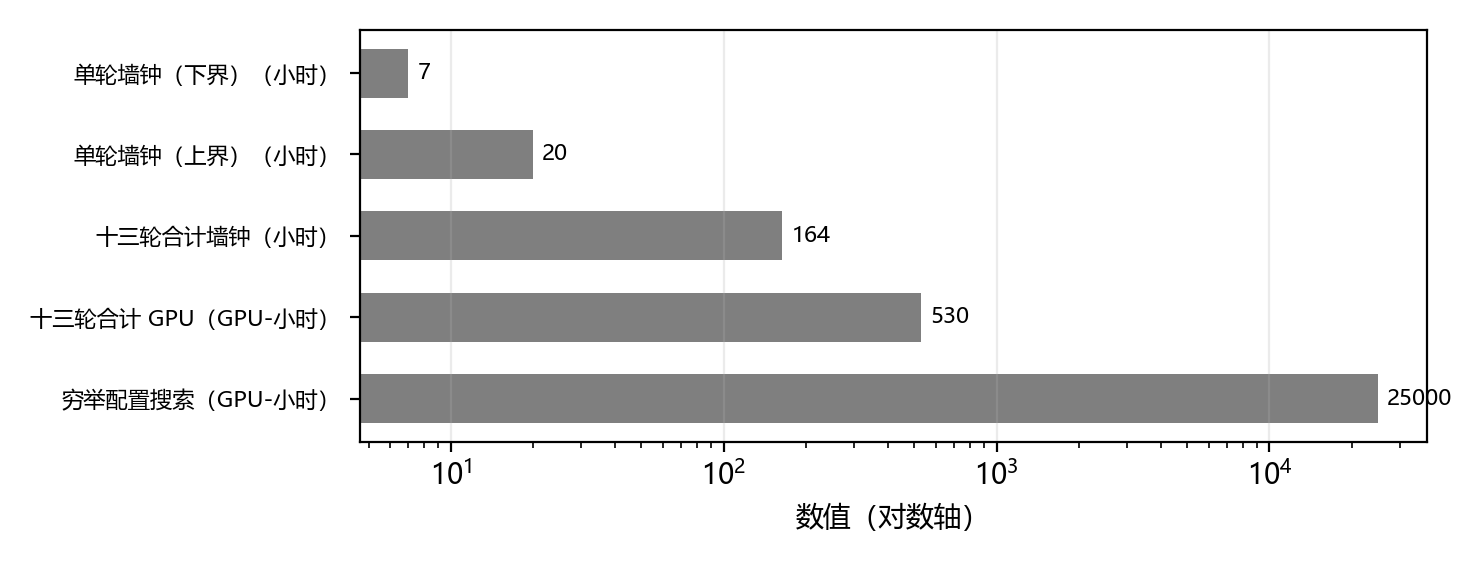
\includegraphics[width=0.86\textwidth]{../figures/fig3_cost.png}
\caption{图 2　循环的代价结构与穷举基线。横轴为对数轴——从 7 小时到 25,000 GPU-小时，跨度三个数量级。}
\label{fig:2}
\end{figure*}

这张图要说的是：端到端层的「自动化」本质上是\textbf{用代理模型换实测}。凡是声称「自动找到更优配置」而不报代理误差与实测校准成本的工作，其结论无法被第三方复核。


\section{边界：机制会反号，测量会骗人}

\subsection{批处理是反号的主要触发器}

三条来自同一篇论文的反号证据{\scriptsize\texttt{[c-\hspace{0pt}boundary]}}：


\begin{table*}[t]
\centering
\footnotesize
\setlength{\tabcolsep}{4pt}
\caption{四种失效条件：前两条来自端到端本身，后两条来自测量方式}
\label{tab:4}
\begin{tabular}{lll}
\toprule
条件 & 机制 & 证据 \\
\midrule
批处理 & 每请求验证工作约翻倍，摊薄收益 & 24 节点树 −14.9\% \\
任务饱和 & 已到顶的系统测不出差别 & 比较失效 \\
平均情况代理 & 解析近似扭曲 SLA，甚至反转结论 & 模拟器论文自述 \\
离线 autotune 假设 & MoE 下最优配置取决于路由分布 & 1.45x 差距 \\
\bottomrule
\end{tabular}
\end{table*}

\begin{figure*}[t]
\centering
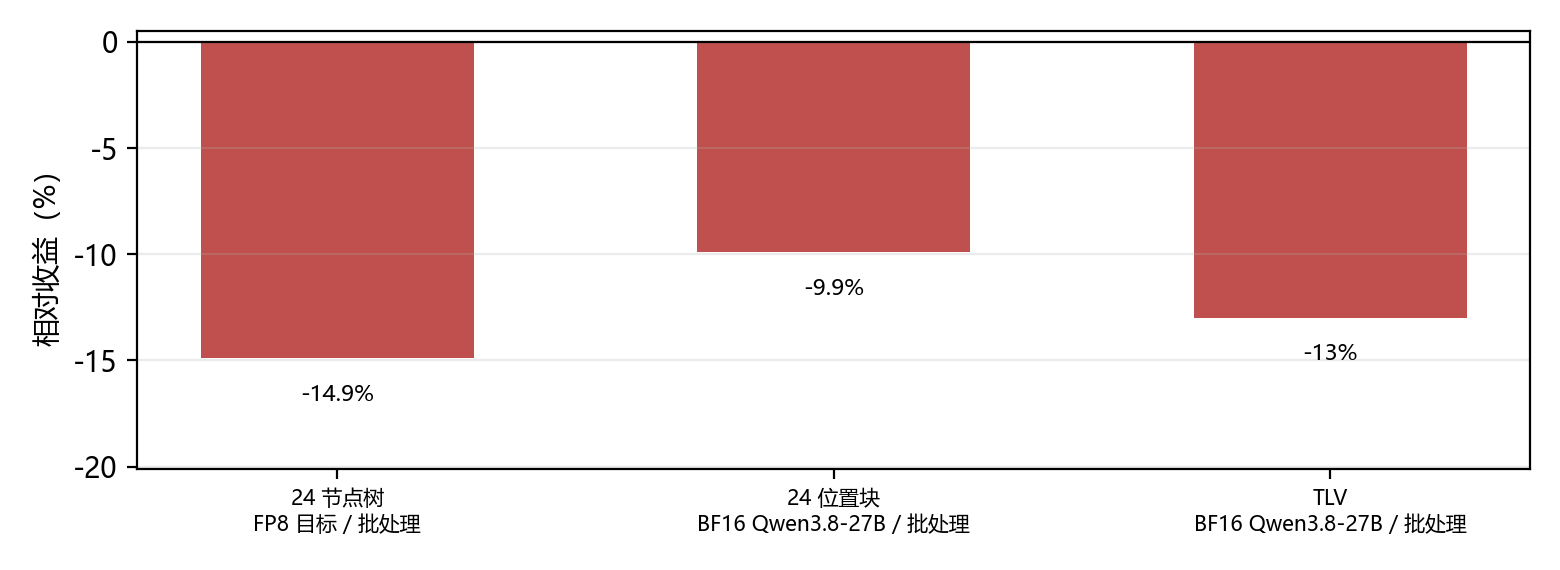
\includegraphics[width=0.86\textwidth]{../figures/fig4_reversal.png}
\caption{图 3　机制反号：三条都在批处理条件下由正转负。}
\label{fig:3}
\end{figure*}

\subsection{测量本身的四种失效}

有一篇工作把「测量不可信」本身做成了研究对象，从四天、619 次模型调用的试点语料里归纳出四种失效模式{\scriptsize\texttt{[c-\hspace{0pt}measure]}}：


\begin{enumerate}
  \item \textbf{稻草人基线制造加速比}：用最差初稿作分母，同一个 kernel 从 2.03 倍读成 10.6 倍{\scriptsize\texttt{[c-\hspace{0pt}measure]}}{\scriptsize\texttt{[c-\hspace{0pt}judge]}}。
  \item \textbf{绝对值不可跨机器迁移}：同一配置 1.174 倍对 1.0049 倍{\scriptsize\texttt{[c-\hspace{0pt}judge]}}。
  \item \textbf{任务饱和使比较失效}：已经到顶的系统再怎么改都测不出差别{\scriptsize\texttt{[c-\hspace{0pt}boundary]}}。
  \item \textbf{基础设施缺陷冒充科学}：机器故障、缓存污染等被当成改进或退化。
\end{enumerate}

\begin{table*}[t]
\centering
\footnotesize
\setlength{\tabcolsep}{4pt}
\caption{最小报告清单：缺任一项，端到端的「改进率」就无法被第三方复核}
\label{tab:5}
\begin{tabularx}{\textwidth}{lX}
\toprule
项 & 为什么必须写 \\
\midrule
基线是什么 & 稻草人基线可制造 10.6x vs 2.03x \\
是否配对运行 & 跨机器绝对值从 1.174x 漂到 1.0049x \\
是否有下界 & 点估计无法区分改进与噪声 \\
无损怎么判 & 逐位相同会误杀，准确率会漏放 \\
循环成本 & 530 GPU-小时换来的结论与免费结论不等价 \\
\bottomrule
\end{tabularx}
\end{table*}

\section{讨论：这是 RSI 吗？}

\subsection{三条判据}

把「递归自我改进」拆成可检验的三条：


\begin{enumerate}
  \item \textbf{改进是否随时间加速？} 若加速，回报曲线应上凸。
  \item \textbf{改进是否作用于改进者自身？} 若只作用于被优化对象，那是自动优化。
  \item \textbf{改进是否可累积、可迁移？} 若每次从零开始，那是测试时扩展。
\end{enumerate}

逐条对照证据：


\begin{itemize}
  \item 第 1 条：\textbf{证据不足}。本文核到的工作普遍只报终点值，只有少数给了逐轮轨迹；没有一条给出「增益随轮次递增」的曲线。
  \item 第 2 条：\textbf{部分是}。端到端改的是系统设计（调度、精度、算法形状），而改进这些设计的 agent 没有被改。
  \item 第 3 条：\textbf{是，但范围有限}。晋级机制被封成带代码增量、正确性契约与未测工况的记忆条目{\scriptsize\texttt{[c-\hspace{0pt}memory]}}，且在同一系统上「在早期会话上继续」优于独立重试{\scriptsize\texttt{[c-\hspace{0pt}memory]}}。
\end{itemize}

\textbf{结论：端到端层目前是「判据已工程化的自动优化」，不是递归自我改进。}


\subsection{一次反证：脚手架自改进其实很弱}

第三节把「可累积性」判为「是」，但有一组实证把这个「是」压得很低。


一个针对编码 agent 的研究收集了 125 条 harness 改动提议，实现了 24 条，评估了 12 条；在 7 次「新会话确实遇到目标问题」的评估里，\textbf{2 次消除了目标动作、1 次减少、4 次没有减少}，还有一些改动给无关问题增加了工作量{\scriptsize\texttt{[c-\hspace{0pt}harness]}}。


\begin{figure*}[t]
\centering
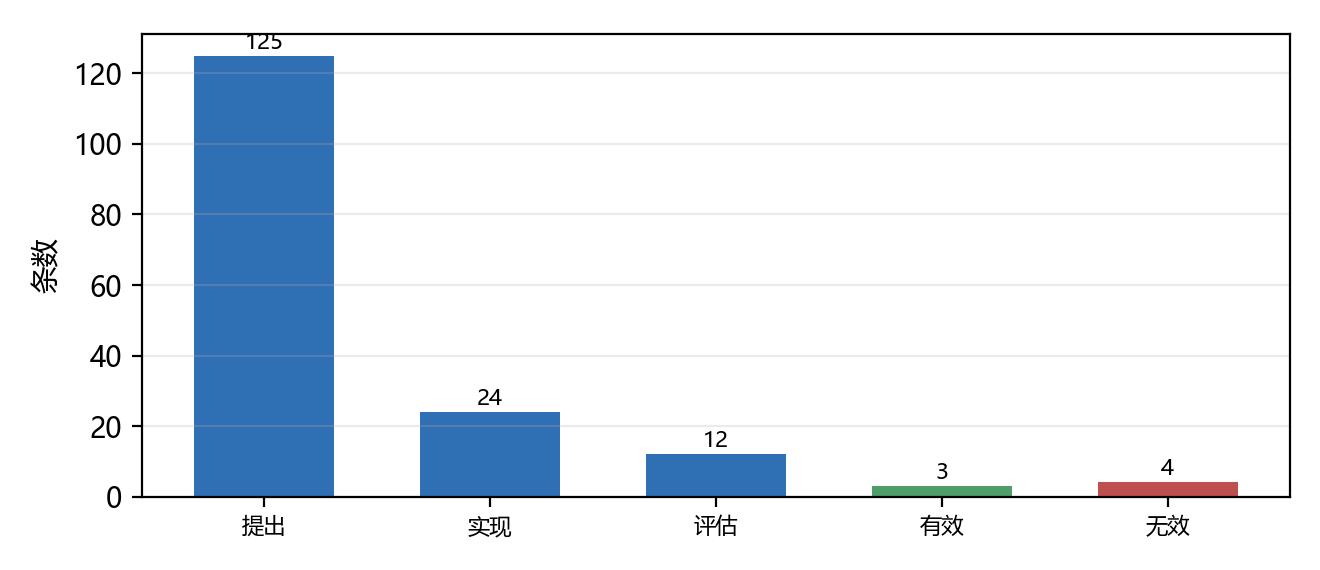
\includegraphics[width=0.86\textwidth]{../figures/fig2_funnel.png}
\caption{图 4　脚手架自改进的漏斗：125 条提议 \sym{→}{} 24 条实现 \sym{→}{} 12 条评估 \sym{→}{} 3 条有效。}
\label{fig:4}
\end{figure*}

\begin{table*}[t]
\centering
\footnotesize
\setlength{\tabcolsep}{4pt}
\caption{harness 自改进的漏斗：提议到有效，衰减约 40 倍}
\label{tab:6}
\begin{tabular}{lrl}
\toprule
阶段 & 数量 & 说明 \\
\midrule
提议 & 125 & 一次回顾会话产出的 harness 改动建议 \\
实现 & 24 & 真正落地的改动 \\
评估 & 12 & 在新会话里做 A/B 的改动 \\
有效 & 3 & 2 次消除、1 次减少目标重复工作 \\
无效 & 4 & 7 次可评估改动中没有减少 \\
\bottomrule
\end{tabular}
\end{table*}

这是本文对「RSI」这个名字最直接的反证：\textbf{如果连「改自己的脚手架」都只有不到一半的改动真的有用，那么「自我改进」目前更像是一个有待实现的目标，而不是一个已经观测到的现象。}


\subsection{为什么「自我改进」与「检索已知配方」难以区分}

还有一个更麻烦的问题。开放式端到端基准的设计者自己承认：\textbf{名义上开放的任务，往往可以通过检索一个众所周知的配方再调几个超参来解决}，于是高分既可能来自真优化，也可能来自记忆{\scriptsize\texttt{[c-\hspace{0pt}learn]}}。


一个具体信号是：在某个场景下，三个不同的优化器都收敛到同一个已知引擎{\scriptsize\texttt{[c-\hspace{0pt}learn]}}。这不像发现了新方法，更像选对了型。


另一个基准把这个问题推到更硬的位置：serving 知识常常是\textbf{隐式的、未公开的、且随时间变化}的，故静态基准测不出「从经验中自改进」{\scriptsize\texttt{[c-\hspace{0pt}measure]}}。


\subsection{为什么这条路仍然值得走}

一个系统敢于让 agent 生成整个 serving 栈，理由被写得很清楚：\textbf{目标具体且数值化，正确性有参照}{\scriptsize\texttt{[c-\hspace{0pt}learn]}}。这句话是端到端层相对其他领域（如科研发现）的结构性优势——它的判据天然可执行。


本文的批评因此不是「这条路走不通」，而是「这条路目前的判据还不够硬」。


\section{结论}

本文用 23 篇论文、60 条可回溯证据回答了一个比「多快」更窄的问题：\textbf{端到端的循环用什么判据才敢说「改进了」。}


由此得到四条结论：


\textbf{第一，端到端的对象是「系统设计 + 运行时状态」，判据必须覆盖吞吐、数值正确与部署约束三者。} 同一个 kernel 的最优配置取决于路由分布，故循环必须在运行时闭合{\scriptsize\texttt{[c-\hspace{0pt}object-\hspace{0pt}e2e]}}{\scriptsize\texttt{[c-\hspace{0pt}boundary]}}。


\textbf{第二，「改进」必须是统计命题。} 点估计在跨机器漂移（1.174 对 1.0049）与基线选择（10.6 对 2.03）面前不成立，可行判据只有「下界对噪声」{\scriptsize\texttt{[c-\hspace{0pt}judge]}}。


\textbf{第三，「无损」不能用逐位相同也不能用准确率。} 可行判据是「精确 pass 的 argmax」加上相对基线的失配率统计检验{\scriptsize\texttt{[c-\hspace{0pt}lossless]}}。


\textbf{第四，主要风险是测不准，不是搜不到。} 四种测量失效模式与三种机制反号说明：端到端层的多数「改进」需要先被证明不是测量假象{\scriptsize\texttt{[c-\hspace{0pt}measure]}}{\scriptsize\texttt{[c-\hspace{0pt}boundary]}}。


\subsection{可迁移的三条判据工程}

撇开命名之争，本文认为有三条做法值得迁移到别的优化对象上{\scriptsize\texttt{[c-\hspace{0pt}transfer]}}：


\begin{enumerate}
  \item \textbf{先用最便宜的证据估 headroom，再决定是否实现。} 精确重放、微基准、单卡计时，都比重写系统便宜{\scriptsize\texttt{[c-\hspace{0pt}transfer]}}。
  \item \textbf{晋级要允许「单独不够、合起来够」。} 许多补丁单独过不了门槛，但叠起来够——故判据必须能作用于组合，而不只作用于单条改动{\scriptsize\texttt{[c-\hspace{0pt}transfer]}}。
  \item \textbf{把预算显式分配给「改」与「验」两侧。} 每个中间版本都完整评估会耗尽预算，故验证必须是可分配的资源而不是固定的后置步骤{\scriptsize\texttt{[c-\hspace{0pt}transfer]}}{\scriptsize\texttt{[c-\hspace{0pt}transfer]}}。
\end{enumerate}

第 2 条与第 3 条合起来，正好解释了为什么端到端层的创新集中在判据而不是搜索：\textbf{当验证比生成更贵时，聪明的做法是少验证、验证得更准，而不是多试几次。}
